%%%%%%%%%%%%%%%%%%%%%%%%%%%%%%%%%%%%%%%%%%%%%%%%%%%%%%%%%%%%%%%%%%%%%%%%%%%%%%%%
%%%%%%%%%%%%%%%%%%%%%%%%%%%%%%%%%%%%%%%%%%%%%%%%%%%%%%%%%%%%%%%%%%%%%%%%%%%%%%%%
%%                          AUTHOR: BIBEKANANDA DATTA                         %%
%%                             (C) SEPTEMBER 2023                             %%
%%                      PHD STUDENT, MECHANICAL ENGINEERING                   %%
%%                           JOHNS HOPKINS UNIVERSITY                         %%
%%%%%%%%%%%%%%%%%%%%%%%%%%%%%%%%%%%%%%%%%%%%%%%%%%%%%%%%%%%%%%%%%%%%%%%%%%%%%%%%
%%%%%%%%%%%%%%%%%%%%%%%%%%%%%%%%%%%%%%%%%%%%%%%%%%%%%%%%%%%%%%%%%%%%%%%%%%%%%%%%
\documentclass[12pt]{article}



%%%%%%%%%%%%%%%%%%%%%%%%%%%%% LaTeX Packages %%%%%%%%%%%%%%%%%%%%%%%%%%%%

\usepackage[utf8]{inputenc}	    %input
\usepackage[pagewise,mathlines]{lineno}

% math packages
\usepackage{amsfonts,amssymb,amsmath,amsthm,dsfont,mathtools,mathbbol,siunitx,upgreek,mathrsfs,cancel}
\allowdisplaybreaks[1]

\usepackage[ruled]{algorithm2e} % algorithm package
\usepackage[title,titletoc]{appendix}
\usepackage{autobreak}
\usepackage[english]{babel}		% for other languages
\usepackage{blindtext}

% bibliographic package
% make sure your bib file is in BibLaTeX format
\usepackage[backend=biber, style=apa, doi=true]{biblatex}

\usepackage[font=small,labelfont=bf,labelsep=period]{caption}

\usepackage{color}
\usepackage{csquotes}           % for quote envionrment
\usepackage{enumitem}			% list environment
\usepackage{float}              % for image floating
\usepackage[T1]{fontenc}		% output
\usepackage{geometry}		    % margin manipulation

\usepackage{fancyhdr}
\usepackage[bottom]{footmisc}
\usepackage{graphicx,wrapfig}   % for image  
\usepackage{hyperref}

% table related package
\usepackage{booktabs,longtable,makecell,multicol,multirow,tabularx,xltabular}
%\usepackage[protrusion]{microtype}
\usepackage{textcomp}
\usepackage{sectsty}
\usepackage{setspace}
\usepackage{seqsplit}
\usepackage[rightcaption]{sidecap}
\usepackage{soul}
\usepackage{tocbasic,parskip}
\usepackage{parskip}
\usepackage{titlesec}
%\usepackage{tocbibind}
\usepackage{tikz}
\usetikzlibrary{positioning}
\usetikzlibrary{shapes,arrows}
\usepackage{subfig}    % Individual panel captions
\usepackage{xcolor}

%% add more packages as you need

%%%%%%%%%%%%%%%%%%%%%%%%%% END LaTeX Packages %%%%%%%%%%%%%%%%%%%%%%%%%%%



%%%%%%%%%%%%%%%%%%%%%%%% DOCUMENT FORMATTINGS %%%%%%%%%%%%%%%%%%%%%%%%%%%

%% margin settings with geometry package
\geometry{left=1in, right=1.0in, top=1.0in, bottom=1.0in}

%%% table of content, list of table, list of figure header setting with tocbasic
\addtotoclist[\jobname]{toc}
\renewcommand \tableofcontents{\listoftoc[{\contentsname}]{toc}}
\renewcommand*{\listoffigures}{\listoftoc[\listfigurename]{lof}}
\renewcommand*{\listoftables}{\listoftoc[\listtablename]{lot}}
\setuptoc{lof}{totoc}
\setuptoc{lot}{totoc}


%% section, subsection, and subsubsection to appear in the TOC
\setcounter{secnumdepth}{3}


%% formatting for the section, subsection, subsubsection, etc.
\titleformat{\section}
{\large\bfseries}{\thesection}{1em}{}[{\titlerule}]
\titleformat*{\subsection}{\normalsize\bfseries}
\titleformat*{\subsubsection}{\normalsize\itshape}


%% no indent with single paragraph spacing
\baselineskip=12pt
\setlength{\parindent}{0pt}
\setlength{\parskip}{\baselineskip}
\setlength{\footnotesep}{0.75\baselineskip}
\setlength{\marginparwidth}{2.5cm} 
\setlength{\bibitemsep}{0.75\baselineskip}  %% bib item separation 
\def\arraystretch{1.25}
\singlespacing

%% settings for bibliography
\DeclareFieldFormat{titlecase}{#1}
\AtBeginBibliography{\urlstyle{rm}}

%% settings for hyperref package
\hypersetup{linktocpage, unicode, colorlinks=true, citecolor=blue, filecolor=blue, linkcolor=blue, urlcolor=blue}


%% settings for figure caption
\captionsetup{belowskip=0pt}

%%%%%%%%%%%%%%%%%%%%%% END DOCUMENT FORMATTINGS %%%%%%%%%%%%%%%%%%%%%%%%%




%%%%%%%%%%%%%%%%%%%%%% MATH SETTINGS AND MACROS %%%%%%%%%%%%%%%%%%%%%%%%%

%% Define math symbols and macros
\numberwithin{equation}{section}
\newcommand{\vect}[1]{\mathbf{#1}}
\DeclareMathOperator{\tr}{tr}
\DeclareMathOperator{\divg}{div}
\DeclareMathOperator{\grad}{grad}
\DeclareMathOperator{\curl}{curl}
\DeclareMathOperator{\sym}{sym}
\DeclareMathOperator{\skw}{skw}
\newcommand{\dC}{$^{\circ}$C}

%% these are just some examples. add more macros as you need

%%%%%%%%%%%%%%%%%%%%%% MATH SETTINGS AND MACROS %%%%%%%%%%%%%%%%%%%%%%%%%%



%%%%%%%%%%%%%%%%%%%%%% SIMPLE COMMENT SETTINGS %%%%%%%%%%%%%%%%%%%%%%%%%%

%% for basic commenting purposes (you can add more)
\newcommand{\COMMENT}{\textcolor{red}}
\newcommand{\ADDCITATION}{\COMMENT{(ADD CITATION)}}
\newcommand{\ADDFIGURE}{\COMMENT{(ADD FIGURE)}}
\newcommand{\ADDTABLE}{\COMMENT{(ADD TABLE)}}

%% to add quotes
\newcommand{\say}[2]{\hfill\small\enquote{\textit{#1}}{ - \small\textsc{#2}.}}

%% you can use other packages for more complicated review and comment section

%%%%%%%%%%%%%%%%%%%% END SIMPLE COMMENT SETTINGS %%%%%%%%%%%%%%%%%%%%%%%%




%%%%%%%%%%%%%%%%%%%%%%%%%%% BASIC SETTINGS %%%%%%%%%%%%%%%%%%%%%%%%%%%%%%

%% font (comment one of the following)
\usepackage{lmodern}    	    %latin modern font
%\usepackage[sc]{mathpazo}
%\usepackage{times}             %times new roman

%% may be useful during drafting
%\linenumbers

%% I use Zotero to generate BibLaTeX file and include it in the same directory
\addbibresource{proposal_references.bib}

%%%%%%%%%%%%%%%%%%%%%%%%% END BASIC SETTINGS %%%%%%%%%%%%%%%%%%%%%%%%%%%%


\begin{document}


%%%%%%%%%%%%%%%%%%%%%%%%%%%%% FRONT MATTER %%%%%%%%%%%%%%%%%%%%%%%%%%%%%




%%%%%%%%%%%%%%%%%%%%%%%%%%% BEGIN TITLE PAGE %%%%%%%%%%%%%%%%%%%%%%%%%%%



\vspace*{0.025in}
\thispagestyle{empty}

\begin{center}
    Doctoral dissertation proposal submitted to the \\
    Department of Mechanical Engineering of The Johns Hopkins University \\
    
    \vspace{0.75in}

    \MakeUppercase{\textbf{LOREM IPSUM DOLOR SIT AMET\\CONSECTETUER ADIPISCING ELIT}}       %% tentative thesis title
    
    \vspace{0.25in}
    
    Author name   % AUTHOR (student) NAME
\end{center}

\vspace{0.75in}



%%%%%%%%%%%%%%%%%%%%%%%%%%%% COMMITTEE MEMBERS %%%%%%%%%%%%%%%%%%%%%%%%%%%

% if you have more people on your committee then squeeze out some spaces or use the minipage feature
\begin{singlespace}

    \textbf{Primary advisor:}
    
    Dr. Chuck Darwin \\
    Professor \\
    Department of Biology \\
    Johns Hopkins University, Baltimore, MD \\

    \textbf{Dissertation proposal committee members:} 
    
    Dr. Albrecht Einstein \\
    Professor\\
    Department of Biology \\
    Johns Hopkins University, Baltimore, MD
    
    Dr. Stewart Hawking \\
    Professor\\
    Department of Biology \\
    Johns Hopkins University, Baltimore, MD 
    
\end{singlespace}

%%%%%%%%%%%%%%%%%%%%%%%%%% TIME AND LOCATION %%%%%%%%%%%%%%%%%%%%%%%%%%%
\vspace{1in}
\begin{center}
    Baltimore, Maryland \\  % Location
    Month YEAR              % Like May 2023
\end{center}


%%%%%%%%%%%%%%%%%%%%%%%%%%%% END TITLE PAGE %%%%%%%%%%%%%%%%%%%%%%%%%%%%





%%%%%%%%%%%%%%%%%%%%%%%%%%%% BEGIN ABSTRACT %%%%%%%%%%%%%%%%%%%%%%%%%%%%
\newpage
\pagenumbering{roman}
\setcounter{page}{2}
\addcontentsline{toc}{section}{Abstract}
\section*{Abstract}
\blindtext

%% write your abstract here



%%%%%%%%%%%%%%%%%%%%%%%%%%%%% END ABSTRACT %%%%%%%%%%%%%%%%%%%%%%%%%%%%%





%%%%%%%%%%%%%%%%%%%%%%% TABLE OF CONTENTS ETC %%%%%%%%%%%%%%%%%%%%%%%%%%
\newpage
\onehalfspacing
\renewcommand{\contentsname}{Table of Contents}
\tableofcontents

\newpage
\listoftables


\newpage
\listoffigures

%%%%%%%%%%%%%%%%%%%%%%%%%% END FRONT MATTER %%%%%%%%%%%%%%%%%%%%%%%%%%




%%%%%%%%%%%%%%%%%%%%%%%%%%% BEGIN MAIN TEXT %%%%%%%%%%%%%%%%%%%%%%%%%%

\newpage
\singlespacing
\pagenumbering{arabic}




%%%%%%%%%%%%%%%%%%%%%%%%%%%%% BACKGROUND %%%%%%%%%%%%%%%%%%%%%%%%%%%%%%

\section{Background and significance}    %% 2 page limit

\blindtext

\begin{figure}[ht]
\begin{center}
    \includegraphics[width=\textwidth, trim={6cm 5cm 6cm 5cm},clip,page=2] {proposal_figures.pdf}
    \caption{Here are some photos of ducks to make you feel happy.}
    \label{fig:ducks}
\end{center}
\end{figure}







%%%%%%%%%%%%%%%%%%%%%%%%%%%%%%% OBJECTIVES %%%%%%%%%%%%%%%%%%%%%%%%%%%%%%

\section{Research objectives}       %% 1 page limit

\blindtext


\phantomsection
\subsection*{Objective 1: Some major objective here}
\addcontentsline{toc}{subsection}{Objective 1: Some major objective here}

\blindtext

%% add more objectives (one objective is not enough you know it)





%%%%%%%%%%%%%%%%%%%%%%% METHODOLOGY AND RESULTS %%%%%%%%%%%%%%%%%%%%%%%%%%

\section{Proposed methodology and results} %% 4 page limit

\subsection{Task 1: Major project task heading here related to objective 1}

\blindtext

\begin{figure}[ht]
\begin{center}
    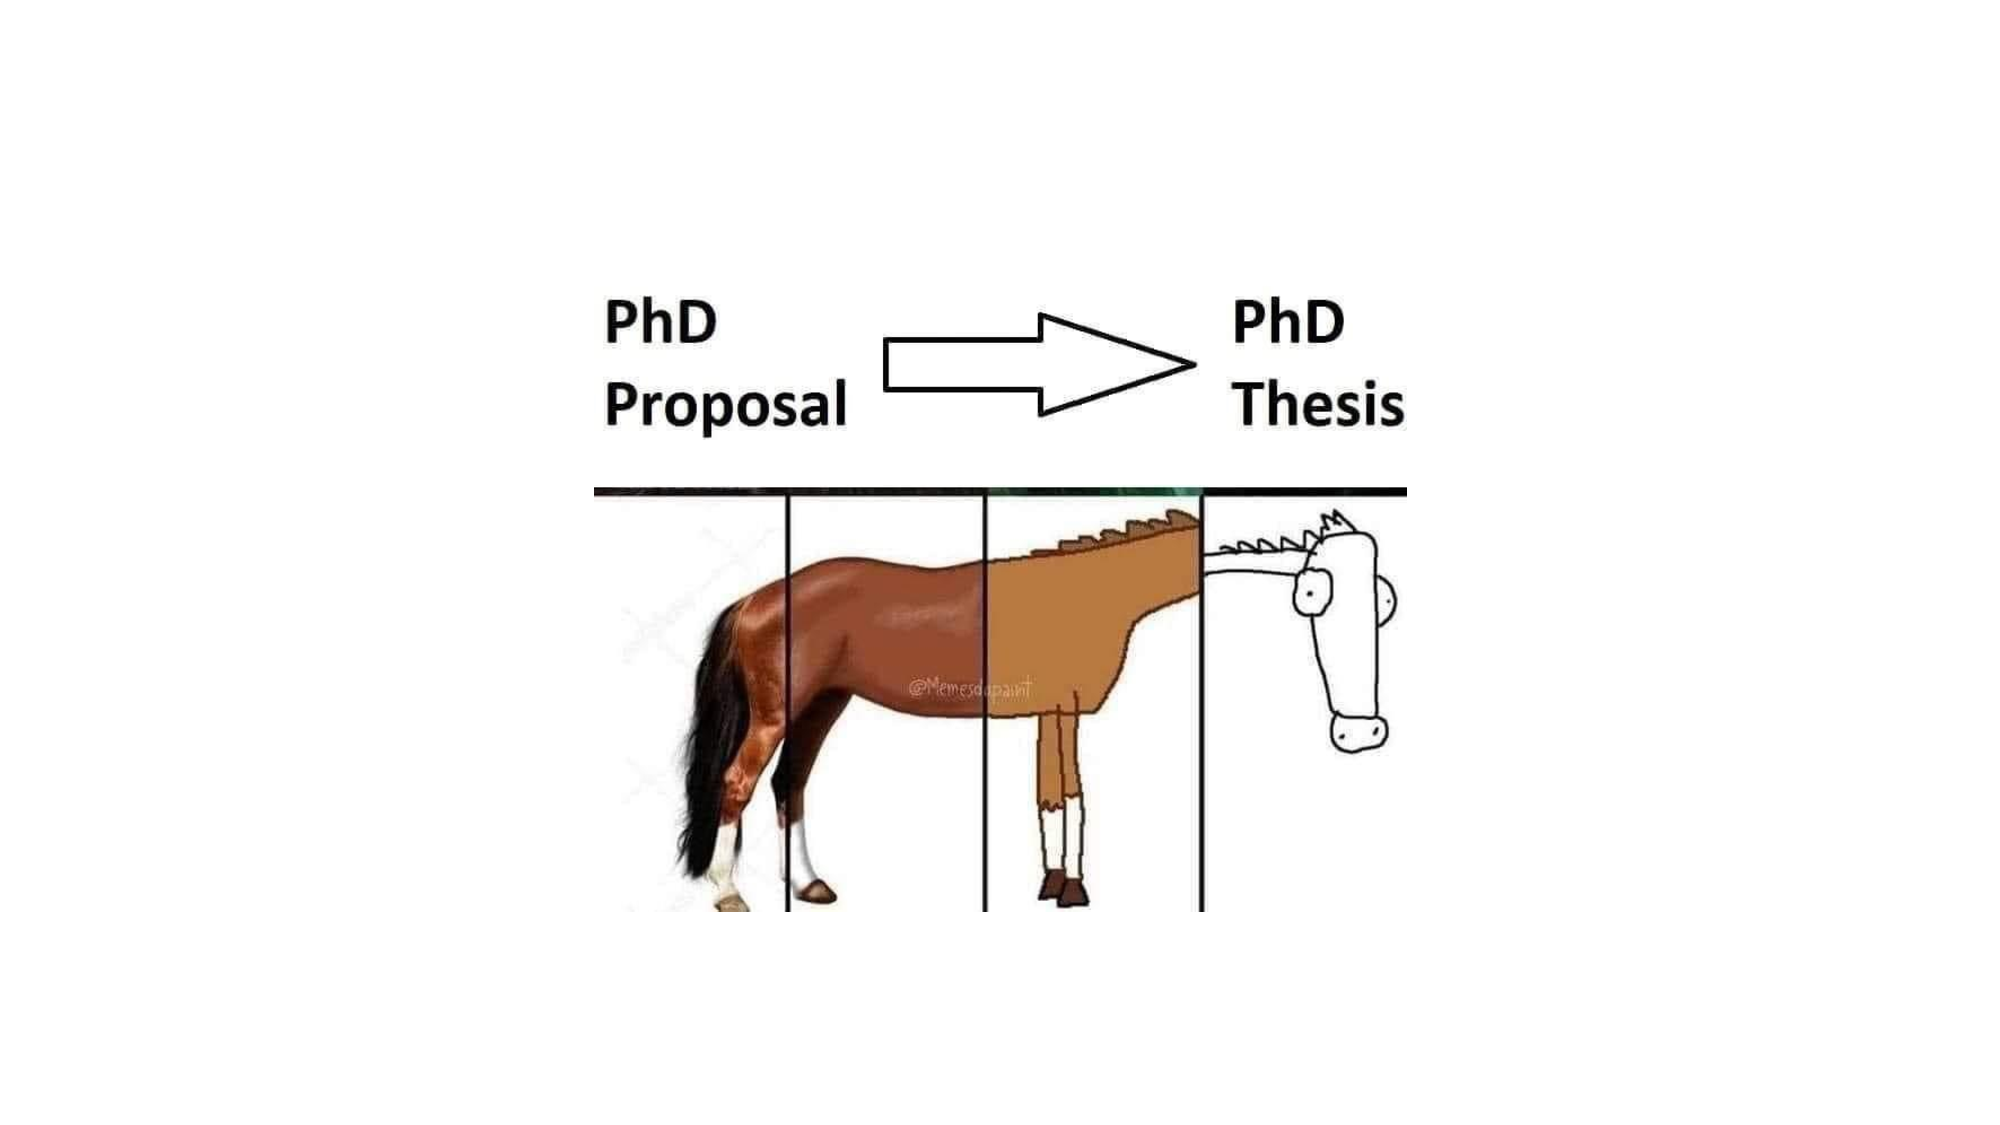
\includegraphics[width=12.5cm, trim={9cm 3cm 9cm 4cm},clip,page=1] {proposal_figures.pdf}
    \caption{Progression of project of a barely surviving PhD student.}
    \label{fig:proposal-plan}
\end{center}
\end{figure}



\subsubsection*{Subtask 1.1: Some sub-task here}
\addcontentsline{toc}{subsubsection}{Subtask 1.1: Some sub-task here}
\blindtext


%% add more tasks and subtasks (one task is not enough for PhD - you know it by now)



%%%%%%%%%%%%%%%%%%%%%%%%%%%%%% PUBLICATIONS %%%%%%%%%%%%%%%%%%%%%%%%%%%%%

\section{Planned publications}

\begin{enumerate} [leftmargin=0.75cm,itemsep=0pt]
    %
    \item %\fullcite{add_the_biblatex_tag}.
    \item %\fullcite{add_the_biblatex_tag}.
    \item %\fullcite{add_the_biblatex_tag}. \hfill (In preparation)
    \item %\fullcite{add_the_biblatex_tag}. \hfill (In preparation)
    %% add more items if you
\end{enumerate}





%%%%%%%%%%%%%%%%%%%%%%%%%%%%%%% TIMELINE %%%%%%%%%%%%%%%%%%%%%%%%%%%%%%%

\section{Timeline}

%% add a chart/ table/ list showing the progress and tentative timelines







%%%%%%%%%%%%%%%%%%%%%%%%%%%%% ACKNOWLEDGEMENT %%%%%%%%%%%%%%%%%%%%%%%%%%%%

%% Optional acknowledgment section (uncomment if you want to use)
% \section*{Acknowledgement}
% \addcontentsline{toc}{section}{Acknowledgement}





%%%%%%%%%%%%%%%%%%%%%%%%%%%%% BIBLIOGRAPHY %%%%%%%%%%%%%%%%%%%%%%%%%%%

\newpage
\section*{References}
\addcontentsline{toc}{section}{References}
\printbibliography[heading=none] 

%%%%%%%%%%%%%%%%%%%%%%%%%%% END BIBLIOGRAPHY %%%%%%%%%%%%%%%%%%%%%%%%%


%%%%%%%%%%%%%%%%%%%%%%%%%%%% END MAIN TEXT %%%%%%%%%%%%%%%%%%%%%%%%%%%




\end{document}